\documentclass[12pt]{article}

% Настройка русского языка и шрифтов
\usepackage[utf8]{inputenc}
\usepackage[russian]{babel}
\usepackage[T2A]{fontenc}

% Математические пакеты
\usepackage{amsmath, amssymb, amsfonts}

% Настройка страницы
\usepackage{geometry}
\geometry{a4paper, margin=0.8in}

% Другие полезные пакеты
\usepackage{hyperref}
\usepackage{booktabs}
\usepackage{enumitem}
\usepackage{longtable}
\usepackage{graphicx}
\usepackage{xcolor}

% Определение стилей для комментариев
\definecolor{commentgray}{rgb}{0.4,0.4,0.4}
\definecolor{antigravityblue}{rgb}{0.0, 0.45, 0.74}

\newcommand{\commentary}[1]{{\small\itshape\color{commentgray} #1}}
\newcommand{\antigravity}[1]{{\small\color{antigravityblue}\textbf{Antigravity:} #1}}

% Настройка ссылок
\hypersetup{
    colorlinks=true,
    linkcolor=blue,
    filecolor=magenta,      
    urlcolor=cyan,
    pdftitle={Глубокий разбор: Метрики качества},
}

\title{Глубокий разбор: Метрики классификации и регрессии}
\author{Твой персональный гид по ML}
\date{\today}

\begin{document}

\subsection{Типология метрик}
\begin{itemize}
    \item \textbf{Офлайновые метрики}: вычисляются на исторических данных (Accuracy, ROC-AUC, MSE). Нужны для быстрой проверки гипотез.
    \item \textbf{Онлайновые метрики}: измеряются в реальном времени через A/B-тесты (CTR, выручка).
\end{itemize}

\commentary{Модель может иметь идеальный ROC-AUC в офлайне, но «просадить» CTR в онлайне.}

\subsection{Функция потерь vs Метрика качества}
\begin{itemize}
    \item \textbf{Функция потерь (Loss)}: инструмент для обучения, \textbf{обязательно} дифференцируема.
    \item \textbf{Метрика}: внешний критерий для оценки успеха, может быть любой.
\end{itemize}

\subsection{Матрица ошибок (Confusion Matrix)}
\begin{table}[h]
\centering
\begin{tabular}{lcc}
\toprule
& \textbf{Истинный Pos} & \textbf{Истинный Neg} \\
\midrule
\textbf{Предсказали Pos} & TP & FP \\
\textbf{Предсказали Neg} & FN & TN \\
\bottomrule
\end{tabular}
\end{table}

\begin{figure}[h]
    \centering
    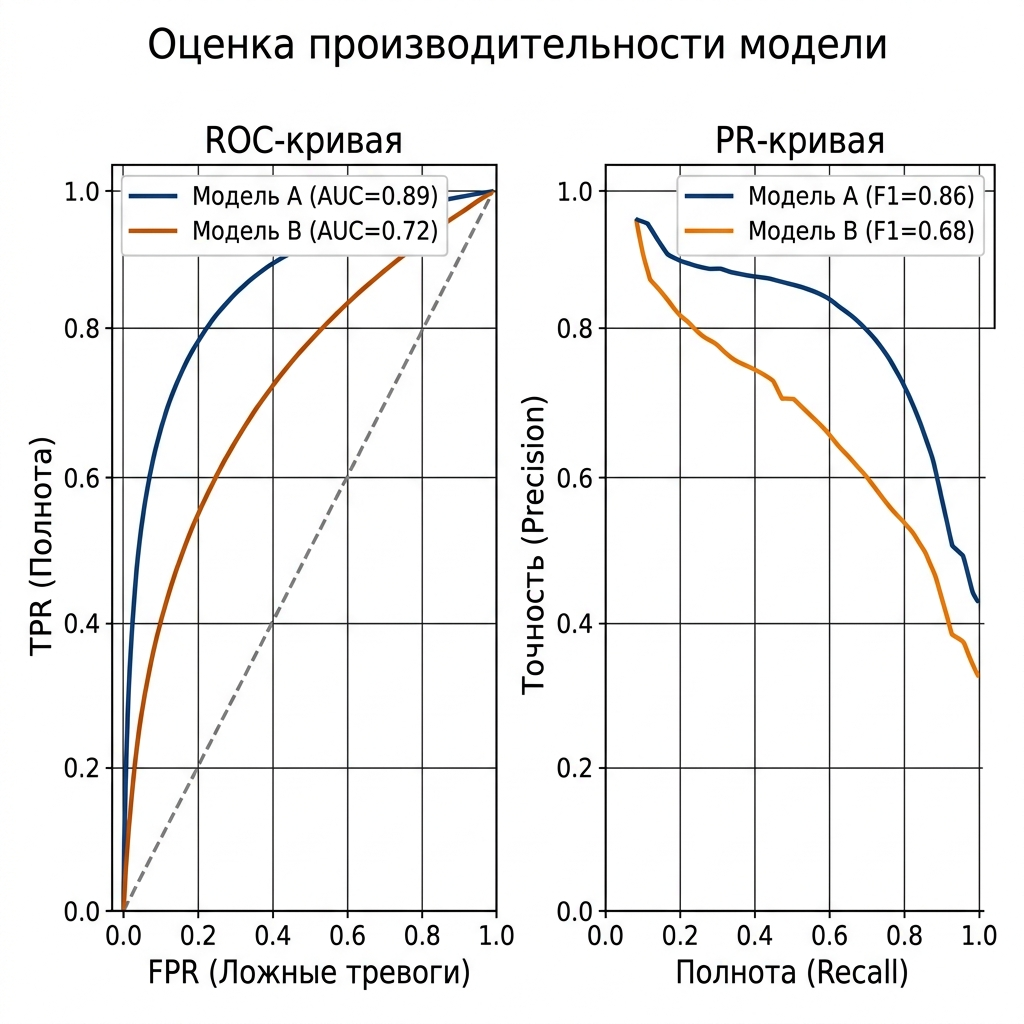
\includegraphics[width=0.7\textwidth]{roc_vs_pr.png}
    \caption{Сравнение ROC и PR кривых.}
\end{figure}

\subsection{Кривые и площади (AUC)}
\begin{itemize}
    \item \textbf{ROC-AUC}: Кривая в осях TPR ($Recall$) и FPR ($\frac{FP}{FP+TN}$). Она показывает способность алгоритма верно упорядочивать объекты. AUC равен доле пар объектов разного класса, которые алгоритм верно ранжировал. Не зависит от дисбаланса классов в плане "формы", но может быть обманчив.
    \item \textbf{PR-AUC}: Кривая в осях Precision и Recall. Явно учитывает количество ложных срабатываний и пропусков. Сильно зависит от доли положительного класса, что делает её предпочтительной при сильном дисбалансе.
\end{itemize}

\subsection{Усреднение в многоклассовых задачах}
\begin{itemize}
    \item \textbf{Микроусреднение (Micro)}: Сначала суммируем элементы матриц ошибок для всех классов, а затем считаем метрику. Важен вклад каждого \textit{объекта}.
    \item \textbf{Макроусреднение (Macro)}: Считаем метрику для каждого класса отдельно, а затем усредняем результаты. Важен вклад каждого \textit{класса} (независимо от его размера).
\end{itemize}

\subsection{Метрики классификации}

\begin{longtable}{lp{0.35\textwidth}p{0.35\textwidth}}
\toprule
\textbf{Метрика} & \textbf{Пример задачи} & \textbf{Где ЗАПРЕЩЕНО} \\
\midrule
Accuracy & Распознавание цифр & Фрод (сильный дисбаланс) \\
Precision & Таргетинг (высокая цена звонка) & Поиск пропавших (важен каждый сигнал) \\
Recall & Диагностика рака (нельзя пропустить) & Спам-фильтр (важные письма не в спам) \\
F1-measure & Поиск в базе знаний & Когда Recall критичнее Precision \\
\bottomrule
\end{longtable}

\begin{figure}[h]
    \centering
    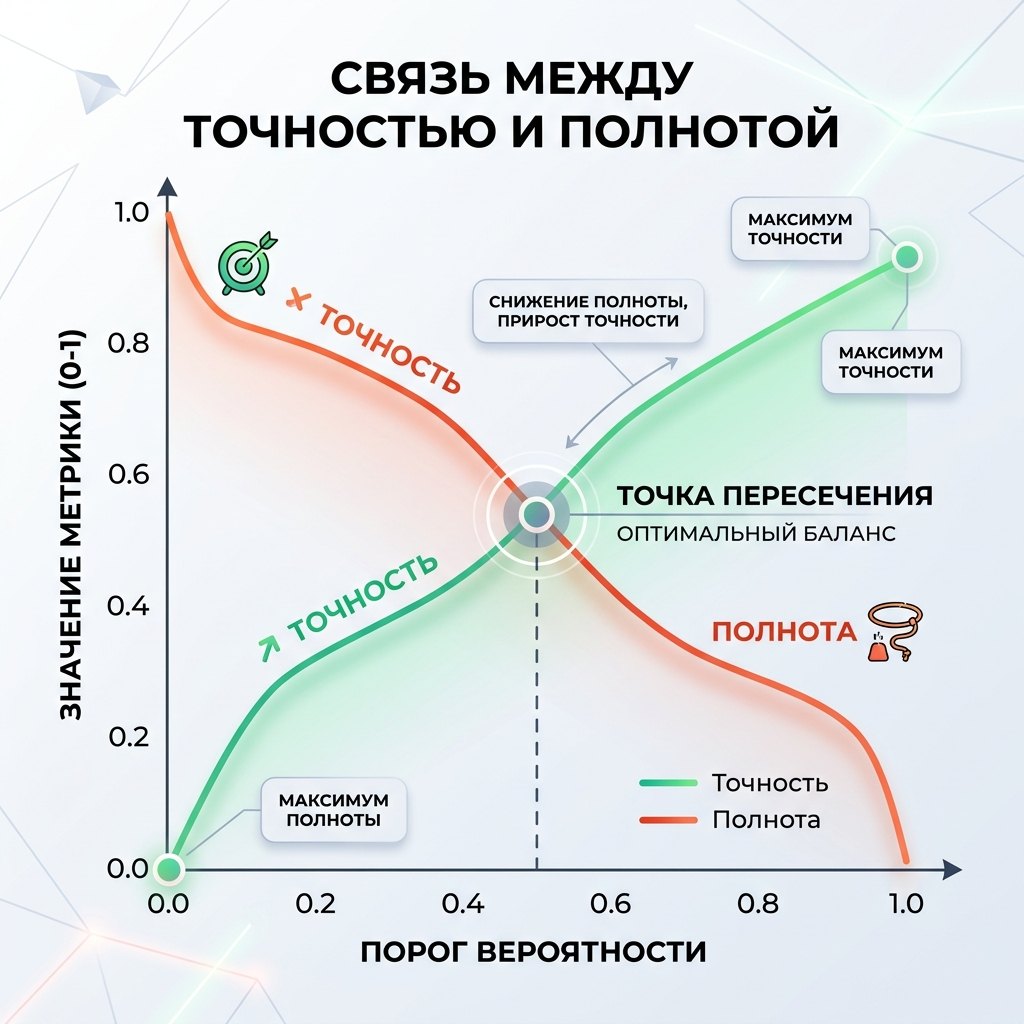
\includegraphics[width=0.6\textwidth]{pr_tradeoff.png}
    \caption{Компромисс между точностью и полнотой.}
\end{figure}

\subsection{Метрики регрессии}

\begin{longtable}{lp{0.35\textwidth}p{0.35\textwidth}}
\toprule
\textbf{Метрика} & \textbf{Пример задачи} & \textbf{Где ЗАПРЕЩЕНО} \\
\midrule
MSE & Нагрузка на сервер (штраф за скачки) & При наличии выбросов \\
MAE & Время доставки (средняя точность) & Когда большие ошибки критичны \\
MAPE & Выручка (понятно бизнесу в \%) & Когда в таргете есть нули \\
SMAPE & Симметричная \% ошибка & Когда важен знак отклонения \\
WAPE & Взвешенная \% ошибка & Когда все объекты равноценны \\
RMSLE & Прогноз цен (важна относительная разница) & Когда важна абсолютная ошибка в рублях \\
\bottomrule
\end{longtable}

\commentary{SMAPE: $\frac{1}{N} \sum \frac{|\widehat{y}_i - y_i|}{(|y_i| + |\widehat{y}_i|)/2}$. WAPE: $\frac{\sum |\widehat{y}_i - y_i|}{\sum |y_i|}$.}

\begin{figure}[h]
    \centering
    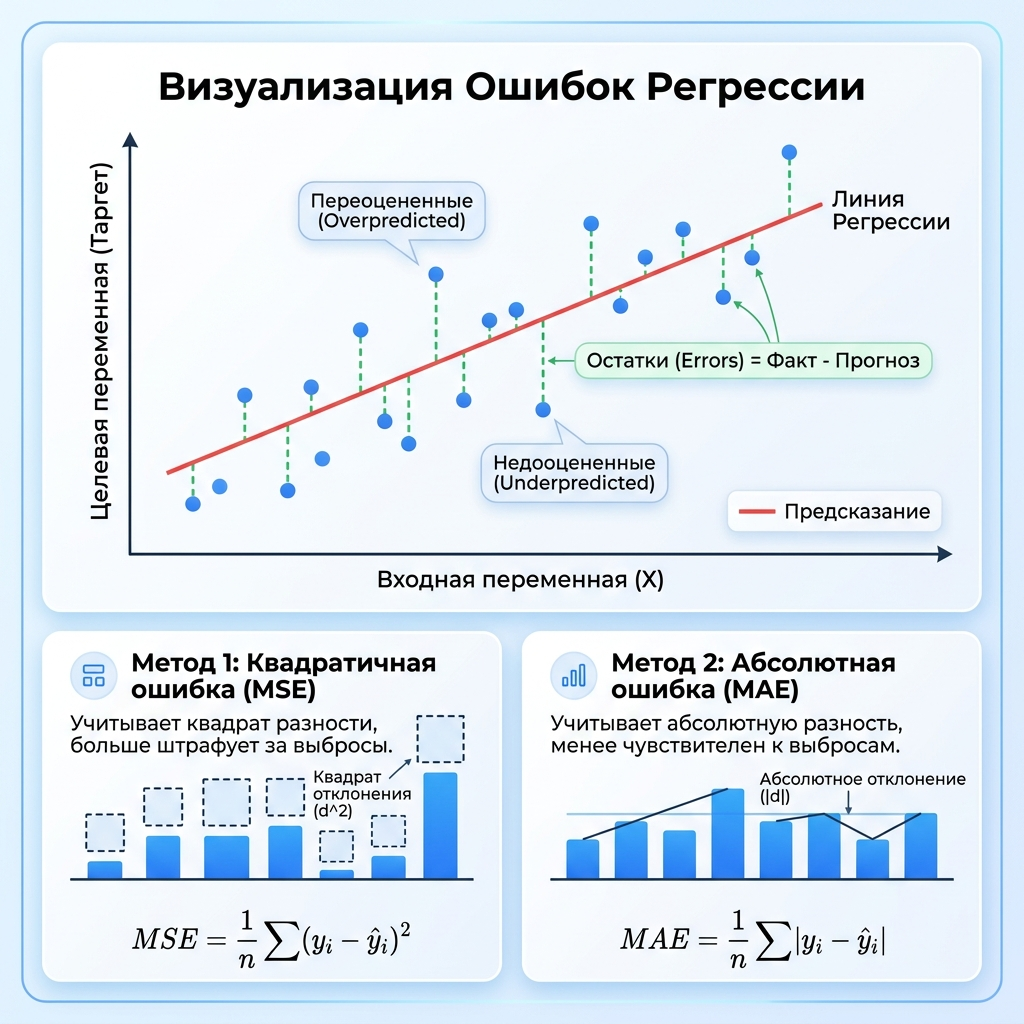
\includegraphics[width=0.7\textwidth]{regression_errors.png}
    \caption{Влияние выбросов на MSE и MAE.}
\end{figure}

\antigravity{Метрики — это мост между бизнесом и математикой. Неверный выбор метрики ведет к созданию идеальной, но бесполезной модели.}

\end{document}
